\begin{frame}{A three state system}
\begin{tabular}{l l}
	\begin{minipage}{0.61\textwidth}
		\begin{block}{Transition rates}
			\begin{equation*}
				\begin{cases}
				k(a,b)=e^{-\beta_1\epsilon}\\
				k(b,a)=1\\
				k(a,c) = 0\\
				k(c,a)=0\\
				k(b,c)=1\\
				k(c,b)=e^{-\beta_2\delta}\\
				\end{cases}
			\end{equation*}
		\end{block}
	\end{minipage}
	&
	\begin{minipage}{0.4\textwidth}
		\begin{figure}
			\centering
			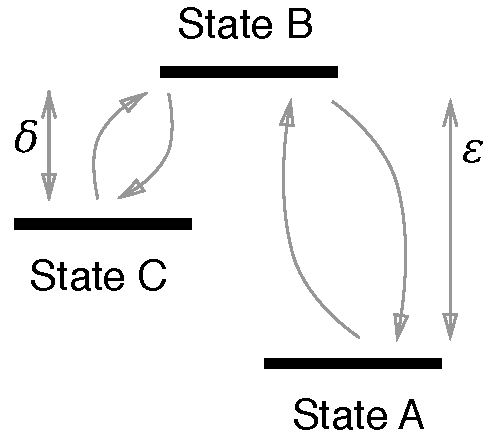
\includegraphics[width=\textwidth]{../src/figure/Simple_3_State_System.pdf}
		\end{figure}
	\end{minipage}
	\end{tabular}
\end{frame}
% % % % % % % % % % % % % % % % % % % % % % % % % % % % % % % % % % % % % % % % %
